\subsection{Hyperparameter Tuning}

Hyperparameter tuning is conducted to assess the sensitivity and
robustness of the proposed two-stage classifier, rather than to
aggressively maximize performance
\subsubsection{Two-Stage Rule Parameters}

We analyze the sensitivity of the Two-Stage classifier to the minimum rule
purity $\tau_p$, minimum rule support $\tau_s$, and the regularization
parameter $C$ of the Stage~2 classifier.

Figure~\ref{fig:purity_f1} shows that macro-averaged F1 increases monotonically
with the rule purity threshold, confirming that selecting highly pure patterns
consistently improves performance.

\begin{center}
	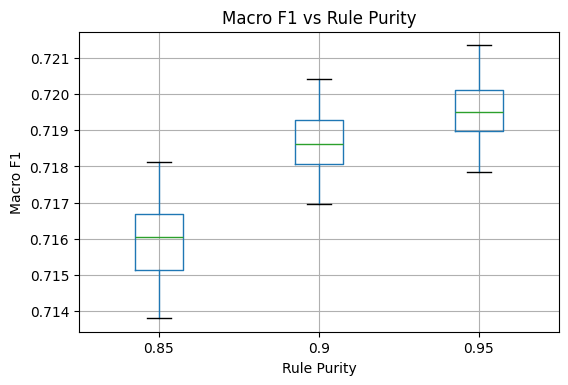
\includegraphics[width=0.7\linewidth]{FIGURES/F1_vs_RulePuriti.png}
	\captionof{figure}{Macro-averaged F1 score as a function of the rule purity threshold $\tau_p$.}
	\label{fig:purity_f1}
\end{center}

Figure~\ref{fig:support_f1} shows that performance remains largely stable across
a broad range of rule support thresholds, indicating limited sensitivity to
$\tau_s$ once sufficiently frequent patterns are retained.

\begin{center}
	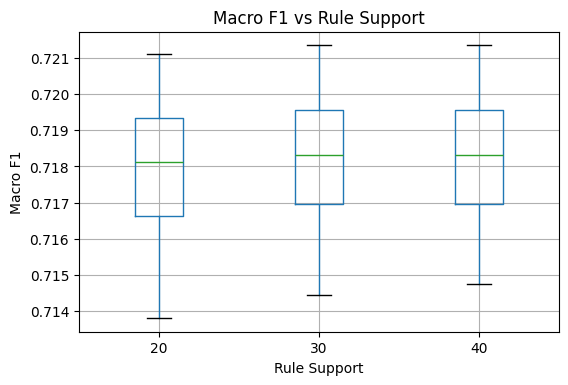
\includegraphics[width=0.7\linewidth]{FIGURES/F1_vs_RuleSupport.png}
	\captionof{figure}{Macro-averaged F1 score as a function of the rule support threshold $\tau_s$.}
	\label{fig:support_f1}
\end{center}

\paragraph{Linear Model Regularization}
The regularization parameter $C$ of the Stage~2 linear classifier is varied
across a wide range. As shown in Figure~\ref{fig:f1_vs_c}, macro-F1 remains
stable for moderate values of $C$, with only marginal degradation for larger
values.

\begin{center}
	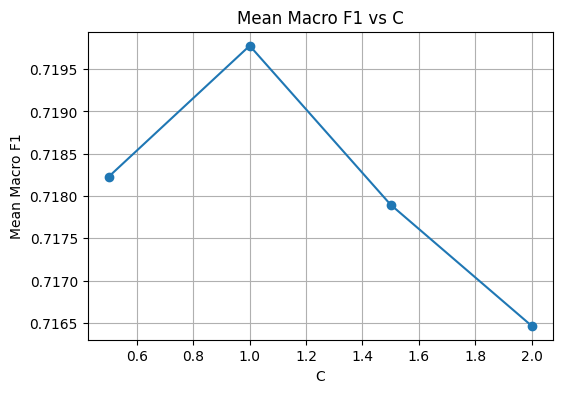
\includegraphics[width=0.7\linewidth]{FIGURES/macro_F1_vs_C.png}
	\captionof{figure}{Macro-averaged F1 score as a function of the regularization
	parameter $C$ for the Stage~2 classifier.}
	\label{fig:f1_vs_c}
\end{center}

\paragraph{Best Configurations}
Table~\ref{tab:best_twostage} reports the top-performing configurations on the
development set, together with the corresponding rule coverage.

\begin{table}[H]
\centering
\caption{Top-performing Two-Stage configurations on the development set.
Reported are the regularization parameter $C$, minimum rule purity $\tau_p$,
minimum rule support $\tau_s$, macro-averaged F1 score, and rule coverage.}
\label{tab:best_twostage}
\small
\begin{tabular}{ccccc}
\hline
\textbf{$C$} & \textbf{$\tau_p$} & \textbf{$\tau_s$} & \textbf{Macro F1} & \textbf{Coverage} \\
\hline
1.0  & 0.95 & 40 & 0.7214 & 0.156 \\
1.0  & 0.95 & 30 & 0.7214 & 0.162 \\
1.0  & 0.95 & 20 & 0.7211 & 0.172 \\
1.0  & 0.90 & 30 & 0.7204 & 0.189 \\
1.0  & 0.90 & 20 & 0.7202 & 0.202 \\
\hline
\end{tabular}
\end{table}

Overall, the results reveal a wide performance plateau across all considered
hyperparameters, indicating that the gains achieved by the Two-Stage approach
are driven by its structural decomposition rather than by fragile tuning.
